\section{Conclusion}


In this paper, we propose a method to enable faster and better learning by combining the skills learned in the pretrain phase.
The interesting thing is that it is better to have a skill weight regardless of the state than to have a different skill weight for each state.
Based on these results, we want to find a way to better utilize skill combinations such as attention in the future.



% \subsection{Attention}
\begin{figure}[hb]
  \vskip 0.2in
  \begin{center}
  \centerline{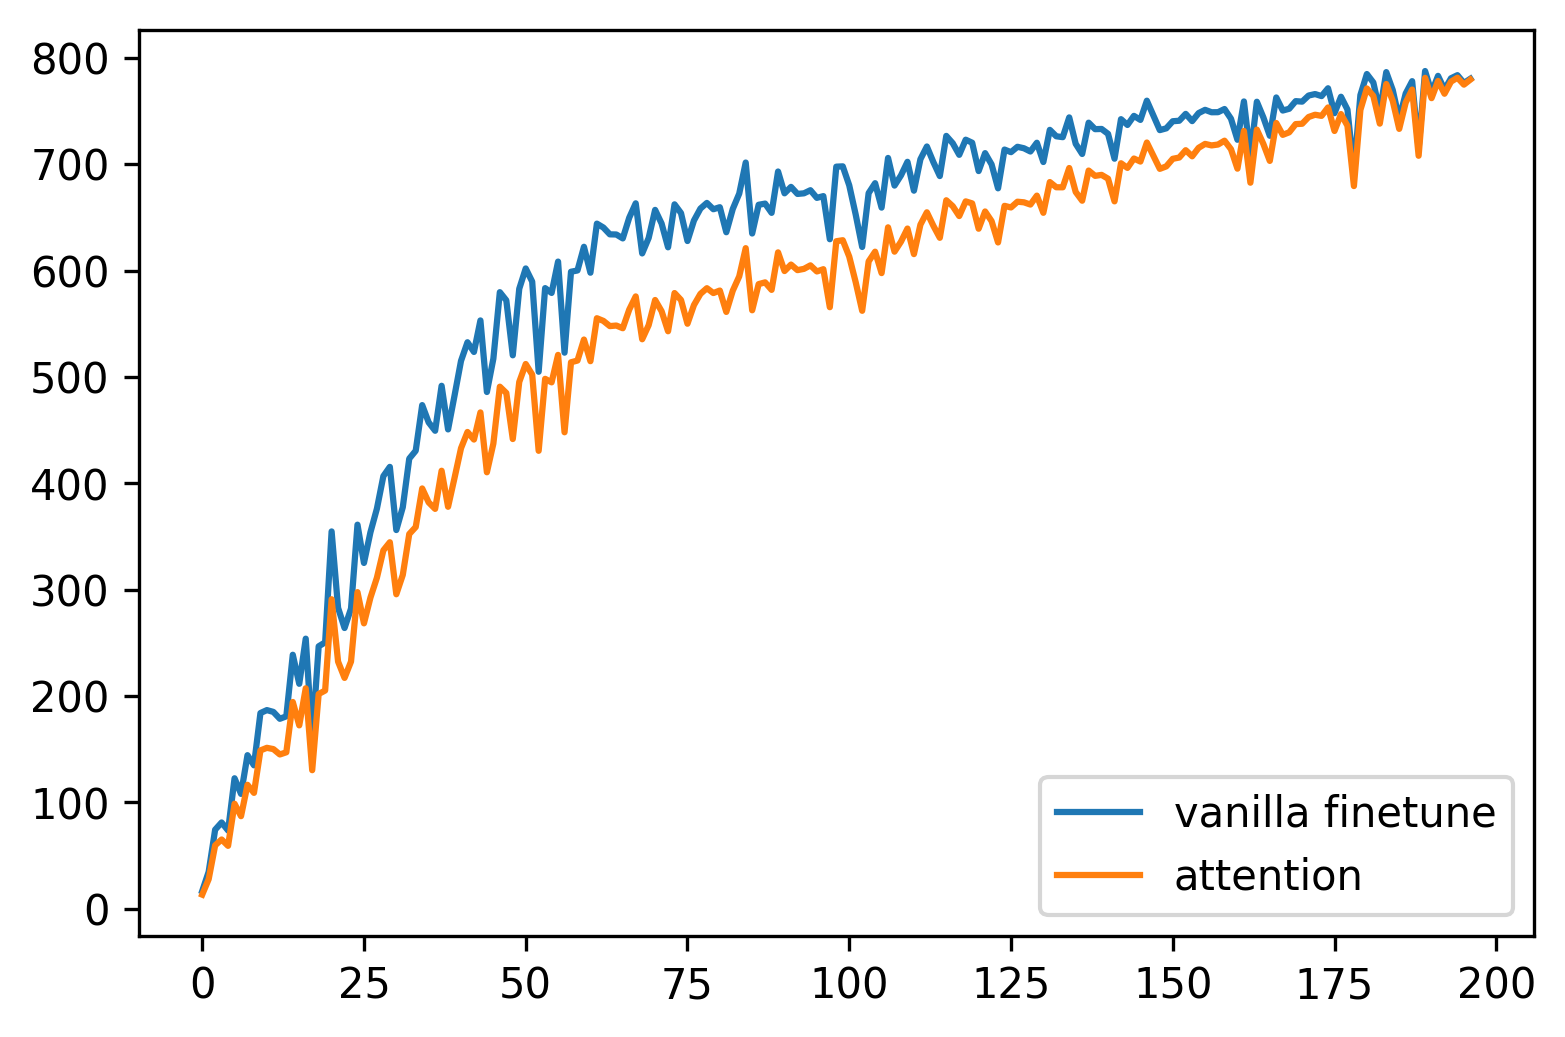
\includegraphics[width=\columnwidth]{Figures/attention_on_walker_run.png}}
  \caption{This result was lost}
  \label{attention-on-walker-run}
  \end{center}
  \vskip -0.2in
  \end{figure}